\openleft%
\chapter[Quantum dot-like plasmonic modes in twisted bilayer graphene supercells][Quantum dot-like plasmonic modes in twisted bilayer graphene supercells]{Quantum dot-like plasmonic modes in twisted bilayer graphene supercells}\label{ch:mat22}
% \chapter[\MultilineTitle{Quantum dot-like plasmonic modes in twisted bilayer graphene supercells}][Quantum dot-like plasmonic modes in twisted bilayer graphene supercells]{Quantum dot-like plasmonic modes in twisted bilayer graphene supercells}\label{ch:mat22}

% \author{T. Westerhout}
% \author{M. I. Katsnelson}
% \author{M. R\"osner}
% \email{m.roesner@science.ru.nl}
% \affiliation{Institute for Molecules and Materials, Radboud University, Heijendaalseweg  135, 6525 AJ Nijmegen, The Netherlands}

{\small We derive a material-realistic real-space many-body Hamiltonian for twisted bilayer graphene from first principles, including both single-particle hopping terms for $p_z$ electrons and their long-range Coulomb interaction. By disentangling low- and high-energy subspaces of the electronic dispersion, we are able to utilize state-of-the-art constrained Random Phase Approximation calculations to reliably describe the non-local background screening from the high-energy $s$, $p_x$, and $p_y$ electron states which we find to be independent of the bilayer stacking and thus of the twisting angle. The twist-dependent low-energy screening from $p_z$ states is subsequently added to obtain a full screening model.  We use this modeling scheme to study plasmons in electron-doped twisted bilayer graphene supercells. We find that the finite system size yields discretized plasmonic levels, which are controlled by the system size, doping level, and twisting angle. This tunability together with atomic-like charge distributions of some of the excitations renders these plasmonic excitations remarkably similar to the electronic states in electronic quantum dots. To emphasize this analogy in the following we refer to these supercells as \emph{plasmonic quantum dots}.  Based on a careful comparison to pristine AB-stacked bilayer graphene plasmons, we show that two kinds of plasmonic excitations arise, which differ in their layer polarization. Depending on this layer polarization, the resulting plasmonic quantum dot states are either significantly or barely dependent on the twisting angle. Due to their tunability and their coupling to light, these plasmonic quantum dots form a versatile and promising platform for tailored light-matter interactions.}

\AdaptedFrom{https://doi.org/10.1088/2053-1583/ac38ca}{T. Westerhout, M. I. Katsnelson, \& M. Rösner,\\2D Materials, 9(1), 014004 (2021).}
\clearpage


\section{Introduction}

\lettrine[lines=3]{L}{ayered} materials with weak interlayer van der Waals (vdW) interactions allow for precise control of the interlayer twisting angle. The resulting moir\'e potential has been shown to yield fascinating effects. For example, for twisted bilayer graphene a small ``magic angle'' has been theoretically predicted, at which ultra-flat bands form~\cite{suarez_morell_flat_2010,bistritzer_moire_2011}. Together with sizable Coulomb interaction this allows for possibly strong correlation effects. Both the characteristics of ultra-flat bands~\cite{li_observation_2010} and the correlation effects have been experimentally verified in the form of insulating and superconducting gaps and in the form of ferromagnetic behavior controlled by doping~\cite{cao_correlated_2018,cao_unconventional_2018,yankowitz_tuning_2019,sharpe_emergent_2019}. For twisted semiconducting layered materials, such as transition metal dichalcogenides (TMDCs), the effects of the moir\'e potential on the excitonic properties have been theoretically~\cite{wu_topological_2017,danovich_localized_2018,wu_hubbard_2018,brem_tunable_2020,choi_twist_2021} and experimentally~\cite{tran_evidence_2019,seyler_signatures_2019,zhang_twist-angle_2020} studied. In these cases, a finite twisting angle can yield superlattices with periodicities of the order of the excitonic radii, which can again yield flat electronic dispersions~\cite{li_imaging_2021,angeli__2021} and can effectively trap exciton complexes~\cite{seyler_signatures_2019,brem_tunable_2020}. 

For both correlation effects in twisted bilayer graphene and the formation of moir\'e excitons in twisted TMDCs, Coulomb interaction plays a major role. While single-particle properties of these twisted materials have been studied in great detail, including the ab initio derivation of the moir\'e potentials, the Coulomb interaction has so far been treated with less care.  For twisted bilayer graphene various models have been utilized ranging from purely local Coulomb interaction~\cite{cao_correlated_2018}, to non-local interaction taking the effective thickness and/or the dielectric environment into account~\cite{goodwin_twist-angle_2019,cea_band_2020,bernevig_twisted_2021,liu_tuning_2021}, and to models treating the low-energy $p_z$ screening on the level of (constrained) Random Phase Approximation~\cite{pizarro_internal_2019,goodwin_attractive_2019}. To describe the Coulomb interaction in twisted bilayer TMDCs, various models have been suggested and used including models resolving the intra- and interlayer Coulomb interactions based on ab initio estimates for the relevant dielectric properties~\cite{danovich_localized_2018,brem_tunable_2020,choi_twist_2021}.

Here, we go beyond these effective Coulomb descriptions by deriving an interacting low-energy model for twisted bilayer graphene including both single-particle and Coulomb interaction matrix elements via state-of-the-art down folding of ab initio calculations.  With this we especially aim to consistently describe the screening from both low-energy $p_z$ orbitals \emph{and} remaining bands, in other words from $sp^2$ and all other higher-energy states.  Although our model remains valid for infinite twisted bilayer graphene structures, we explicitly focus on finite-size supercells and their correlation effects in real space. These finite-size twisted bilayer graphene supercells have been studied in terms of their single-particle properties and optical properties estimated from Fermi's golden rule~\cite{mirzakhani2020circular,tepliakov2020twisted}. Here, we calculate plasmonic excitations in real space for electron-doped finite-size samples at moderate and large twisting angles. So far, plasmons in twisted bilayer graphene have been mostly investigated with a focus on small (``magic'') angles~\cite{sunku_photonic_2018,lewandowski_intrinsically_2019,Hesp_2021_Observation_of,novelli_optical_2020,kuang2021collective} with the exception of Ref.~\cite{hu_real-space_2017}.  Our focus on larger angles comes with a major methodological advantage, which is the circumvention of the screening from extremely flat bands and thus large density of states, as it is in the latter situation still not entirely clear whether the Random Phase Approximation is applicable~\cite{katsnelson_anomalies_1985,irkhin_robustness_2002,stepanov_coexisting_2021}. Additionally, the interlayer hopping model for large twist angles is less delicate than for small angles. In the latter case one needs to take into account atomic relaxations, either numerically~\cite{shi_large-area_2020} or at the model level by introducing a family of topological defects~\cite{gornostyrev_origin_2020}, both of which make the calculations challenging. For moderate to large twist angles, atomic relaxation effects turn out to be negligible as was shown in Ref.~\cite{wijk_relaxation_2015} using atomistic simulations with realistic carbon potentials. The use of a nominal, purely geometric moir{\'e} structure is therefore justified for larger twist angles. 
    
Within the outlined framework, circumventing common modeling issues, we are able to reliably describe real-space plasmonic excitations from first principles at various doping levels and for moderate to large twisting angles.  We find that finite-size supercells naturally yield a discretization of the plasmonic spectrum, which shows well defined and separated plasmonic levels. These plasmonic levels are efficiently tunable by the system size, doping level, and twisting angle. Based on this and in analogy to electronic quantum dots, we refer to these plasmonic systems formed in twisted bilayer graphene supercells as \emph{plasmonic quantum dots}, although their formation is very different to the one of electronic quantum dots. We discuss in detail the real-space charge distribution of these plasmonic excitations in terms of their in-plane shapes and layer polarization. We find that the latter controls the dependence of the corresponding plasmonic quantum dot state on the twisting angle.

\section{Modeling approach}

\subsection{Hamiltonian and plasmonic properties}

\SideFigure{0.5\textwidth}{0pt}{0.4\textwidth}{\hspace{-10pt}\includegraphics[width=\columnwidth]{handmade/Figure_1.pdf}%
}{Sketch of a twisted bilayer supercell with 3252 atoms, armchair edges, and at $\theta = 10\degree$. The rotation axis is marked in dark grey in the inset and is centered on the A (B) sublattice of the upper (lower) layer.%
}{fig:mat22:sc}
% \begin{figure}
%     \centering
%     % \subimport{./assets}{Figure_1.pgf}
%     \includegraphics[width=0.6\columnwidth]{chapters/2D_Materials_9_1_014004/assets/Figure_1.pdf}
%     \caption{Sketch of a twisted bilayer supercell with 3252 atoms, armchair edges, and at $\theta = 10\degree$. The rotation axis is marked in dark grey in the inset and is centered on the A (B) sublattice of the upper (lower) layer.}
%     \label{fig:mat22:sc}
% \end{figure}
    
We aim to study finite-size twisted bilayer graphene supercells as depicted in Fig.~\ref{fig:mat22:sc}. These are constructed such that for zero twist angle ($\theta=0\degree$) we get an AB (Bernal) stacking. The rotation axis is centered at the upper A sublattice (lower B sublattice), as indicated in the inset of Fig.~\ref{fig:mat22:sc}. The outer boundaries are chosen to be of armchair type. We describe these supercells with a low-energy Hamiltonian for the $p_z$ states,
\begin{align}\label{eq:mat22:hamiltonian}
    H = \sum_{i,j,\sigma} t_{ij} c_{i\sigma}^\dagger c_{j\sigma}
      + \sum_{i} U_{ii} n_{i\uparrow} n_{i\downarrow}
      + \sum_{i>j,\sigma, \sigma'} U_{ij} n_{i\sigma} n_{j\sigma'}\,,
\end{align}
with $i$ and $j$ labeling atomic site positions of (twisted) bilayer graphene. $c_{i\sigma}$ ($c_{i\sigma}^\dagger$) and $n_{i\sigma} = c_{i\sigma}^\dagger c_{i\sigma}$ are $p_z$-orbital annihilation (creation) and orbital occupation number operators, respectively, at site $i$ with spin $\sigma$. $t_{ij}$ and $U_{ij}$ are hopping and density-density Coulomb interaction matrix elements, respectively, which we derive in the following section from ab initio calculations. At this stage we do not explicitly differentiate between the upper and lower layer: $i$ and $j$ label lattice sites in both layers. 

To study plasmonic properties we utilize a real-space version of the Random Phase Approximation (RPA)~\cite{Vonsov2012QuantumSolidS,giuliani_quantum_2005,wang_plasmonic_2015,westerhout_plasmon_2018,jiang_plasmonic_2021} to calculate the Electron Energy Loss Spectra (EELS). We start with the eigen decomposition of $\varepsilon(\omega)$:
\begin{equation*}
    \varepsilon(\omega) = \sum_n \varepsilon_n(\omega) \ket{\phi_n(\omega)} \bra{\phi_n(\omega)} \,,
\end{equation*}
where we order the eigenvalues $\varepsilon_n$ according to $-\operatorname{Im}[1 / \varepsilon_n(\omega)]$. $\varepsilon_1$ is the eigenvalue with the largest $-\operatorname{Im}[1 / \varepsilon_n(\omega)]$ and we call it ``leading''. EELS is defined by
\begin{equation*}
    \operatorname{EELS}(\omega) = 
    -\operatorname{Im}\left[ \frac{1}{\varepsilon_1(\omega)} \right] \,.
\end{equation*}
$\phi_1(r, \omega) = \braket{r | \phi_1(\omega)}$ is the corresponding eigenvector in real space which renders the plasmonic excitation pattern. Within a real-space tight-binding approximation, the RPA dielectric matrix is given by
\begin{equation}\label{eq:mat22:Eps_pz}
    \varepsilon_{ij}(\omega) =
        \delta_{ij} -
        \sum_{k} U_{ik} \Pi_{kj}(\omega)
\end{equation}
with the Coulomb interaction $U_{ik}$ entering the Hamiltonian \eqref{eq:mat22:hamiltonian} and the polarizability function $\Pi_{ij}$ given by
\begin{equation}\label{eq:mat22:Pi_pz}
    \Pi_{ij}(\omega) = 
        2 \cdot \sum_{ab} \psi_{ia}^* \psi_{ib} \psi_{jb}^* \psi_{ja}
        \frac{f_a - f_b}{E_a - E_b - (\omega + i\eta)} \,.
\end{equation}
Here $E_a$, $\psi_{ia} \equiv \psi_{a}(i)$ and $f_a = f(E_a)$ are eigenvalues, eigenvectors and corresponding Fermi-Dirac distribution functions obtained upon diagonalization of the single-particle tight-binding Hamiltonian. $i$, $j$, and $k$ label site indices while $a$ and $b$ label eigenstates of the Hamiltonian. $\eta$ is a small positive constant which we set to $1\,$meV in our calculations. More details on the implementation can be found in Ref.~\cite{westerhout_plasmon_2018}.
% In section~\ref{sec:mat22:app_rpa} we furthermore describe how these real-space RPA calculations can be significantly accelerated by exploiting the sparsity of the involved matrices and making use of modern Graphical Processing Units (GPUs).
In the following we derive all the necessary model parameters from ab initio.
    
\subsection{Ab initio down folding}
    
\begin{figure}
    \centering
    \subimport{./assets}{Figure_2.pgf}
    % \includegraphics[width=0.9\columnwidth]{chapters/2D_Materials_9_1_014004/assets/Figure_2.pdf}
    \caption{a) $sp^2$ and b) $p_z$ projected ab initio Density of States (DOS) of AB-stacked (pinkish red) and AA-stacked (green) bilayer graphene. $\omega=0\,$eV corresponds to the Fermi energy.}
    \label{fig:mat22:ab} 
\end{figure}
    
In order to derive all model parameters for arbitrary twist angles via down folding of first principles calculations we have to make one well justified approximation: only the $p_z$ states will experience the moir\'e potential and thus the twist angle $\theta$.  To stress the validity of this assumption we show in Fig.~\ref{fig:mat22:ab}~a) the $sp^2$-projected Density Functional Theory (DFT) density of states (DOS) of pristine AA-stacked (green) and AB-stacked (pinkish red) bilayer graphene. Their difference is nearly invisible so that we can readily assume that the relative layer rotation does not affect these electronic states. This, of course, does not hold for the $p_z$ states, as is obvious from $p_z$-projected DOS shown in Fig.~\ref{fig:mat22:ab}~b).
            
\normalcaptionwidth
\captionwidth{\linewidth}
\begin{table}[h]
  \centering
  \begin{minipage}[t]{0.45\textwidth}%
    \centering
    \fontsize{8pt}{10pt}\selectfont\vspace{0pt}%
    \begin{tblr}{|c|c|c|c|}
	  \hline
      \SetCell[c=2]{c} Intralayer & & \SetCell[c=2]{c} Interlayer & \\
      \hline
      $r$, \AA & $t_{ij}$, eV & $r$, \AA & $t_{ij}$, eV \\ [0.5ex] 
      \hline\hline
      0 & $-0.991$ & 3.35 & $+0.290$ \\ 
      1.42 & $-2.857$ & 3.64 & $+0.118$ \\
      2.47 & $+0.244$ & 3.64 & $+0.067$ \\
      2.85 & $-0.258$ & & \\
      3.77 & $+0.024$ & & \\
      4.28 & $+0.052$ & & \\
      4.94 & $-0.021$ & & \\
      5.14 & $-0.014$ & & \\
      5.70 & $-0.022$ & & \\
      \hline
    \end{tblr}
  \end{minipage}
  % \hspace{0.03\textwidth}%
  \begin{minipage}[t]{0.35\textwidth}%
    \vspace{5pt}%
    % \centering%
    \innerTableCaption{Intra- and interlayer hopping matrix elements for the $p_z$ Wannier orbitals in AB-stacked bilayer graphene. Due to the four sublattices we get two different values for the next-nearest-neighbor interlayer hopping.}
    \label{tbl:mat22:hoppings}
  \end{minipage}%
\end{table}
\changecaptionwidth
\captionwidth{0.9\linewidth}

Based on this assumption we can derive the single-particle hopping matrix elements $t_{ij}$ for the $p_z$ states via a Wannier construction based on DFT calculations for the AB-stacked bilayer graphene.% (see section~\ref{sec:mat22:app_ab} for details).
We calculate the hopping matrix elements via 
\begin{equation*}
    t_{ij}(\theta=0\degree) = \braket{ w_i | H_\text{DFT}^{AB} | w_j }
\end{equation*}
for the untwisted ($\theta=0\degree$) geometry and using the DFT Hamiltonian together with the $p_z$-like ab initio Wannier functions $w_i(r)$. In Table~\ref{tbl:mat22:hoppings} we list the resulting intralayer and interlayer hopping matrix elements for an interlayer distance of $d=3.35\,$\AA. To account for finite twisting angles on the single-particle level, we utilize a Slater-Koster based interlayer hopping model~\cite{guinea_continuum_2019} $t_\perp(r) = \gamma_0 \operatorname{exp}[-\alpha (r-r_0)]$, which we fit to the interlayer hopping matrix elements from Table~\ref{tbl:mat22:hoppings} to obtain $\gamma_0 = 0.29\,$eV and $\alpha = 5.63\,\text{\AA}^{-1}$. As mentioned above, for small twist angles one would additionally need to account for modulations in the interlayer distance~\cite{wijk_relaxation_2015,shi_large-area_2020,gornostyrev_origin_2020}, but here we are interested in moderate to large twist angles such that the assumption of a purely nominal twisting is adequate.
 
The description of fully screened, retarded and $\theta$-dependent Coulomb interaction $W(\omega, \theta)$ requires more attention. $W(\omega, \theta)$ is defined by 
\begin{align}\label{eq:mat22:W_full}
    W(\omega, \theta) = \frac{v}{1 - v \Pi^\text{total}(\omega, \theta)} \,,
\end{align}
where $v$ is the bare Coulomb interaction. $\Pi^\text{total}(\omega, \theta)$ renders all possible screening processes at a given rotation angle $\theta$ which can be separated into two terms:
\begin{align*}
     \Pi^\text{total}(\omega, \theta) \approx 
         \Pi^{p_z}(\omega, \theta) + \Pi^\text{rest}(\omega = 0),
\end{align*}
with $\Pi^{p_z}(\omega, \theta)$ being the partial polarizability resulting from virtual excitations within the low-energy $p_z$ sub-space. It can be evaluated using Eq.~(\ref{eq:mat22:Pi_pz}). The rest polarizability $\Pi^\text{rest}(\omega = 0)$ describes in principle instantaneous screening processes from virtual excitations from, to, and between non-$p_z$ states (such as $sp^2$ and others). Due to the orthogonality of $p_z$ and $sp^2$ states, the cross-polarization terms between $p_z$ and non-$p_z$ orbitals can be safely neglected~\cite{van_loon_random_2021}. This way, $\Pi^\text{rest}$ effectively describes the screening of a semiconductor with a gap of about $10\,$eV [see Fig.~\ref{fig:mat22:ab}~a)], which renders the  instantaneous approximation valid. Importantly, this renders the background (or rest) polarizability independent of the twist angle. Eq.~(\ref{eq:mat22:W_full}) now reads
\begin{align*}
    W(\omega, \theta) 
    &= \frac{v}{1 - v \left[\Pi^{p_z}(\omega, \theta) + \Pi^\text{rest}(\omega = 0)\right]}\\
    &= \frac{U}{1 - U \Pi^{p_z}(\omega, \theta)}\,, \notag \\
    \text{with} \qquad U &= \frac{v}{1 - v \Pi^\text{rest}(\omega = 0)}
\end{align*}
being the $\theta$-independent background-screened Coulomb interaction, as needed for the evaluation of Eq.~(\ref{eq:mat22:Eps_pz}). We calculate $U$ within the constrained RPA~\cite{cRPA} based on ab initio calculations for AB-stacked bilayer graphene.% (see section~\ref{sec:mat22:app_ab} for details).
This yields discretized $U_{ij}$ with $i$, $j$ labeling AB bilayer graphene lattice positions. To check for the $\theta$ independence of $U$ we compared the local and nearest-neighbor (in and out-of-plane) Coulomb interactions $U_{ij}$ between AB and AA stacked bilayer, finding modifications smaller than $3\%$. For the evaluation of Eq.~\eqref{eq:mat22:Eps_pz} we, however, need to evaluate $U_{ij}$ at other positions resulting from the finite twisting angle $\theta$. To this end, we map the discretized $U_{ij}$ to a continuous model $U(r = r_i - r_j)$. For the latter we choose the analytic image-charge model for the potential within a dielectric slab of height $d$ reading~\cite{keldysh_coulomb_1979,jena_enhancement_2007,emelyanenko_effect_2008,jiang_plasmonic_2021}:
\begin{equation} \label{eq:mat22:image-charge-model}
    U(r) =
        \underbrace{
            \frac{e^2}{\varepsilon_m z_0(r)}
        }_{\mathclap{\substack{\text{Local}\\ \text{screening}}}}
        + \underbrace{
            2 \sum_{n=1}^\infty \frac{e^2 \beta_b^n}{\varepsilon_m z_n(r)}
        }_{\mathclap{\substack{\text{Non-local}\\ \text{screening}}}}
\end{equation}
with $e$ being the elementary charge, $\varepsilon_m$ the dielectric constant of the slab, $z_n(r) = \sqrt{r^2 + \delta^2 + (nh)^2}$, and $\beta_b = (\varepsilon_m - 1) / (\varepsilon_m + 1)$. An additional parameter $\delta$ allows us to also fit the on-site potential $U_{ii} = U(r=0)$. In Fig.~\ref{fig:mat22:Coulomb} we show the ab initio cRPA data together with the fit using Eq.~\eqref{eq:mat22:image-charge-model}, the locally-screened interaction $\frac{e^2}{\varepsilon_m z_0(r)}$ ($h \rightarrow \infty$), and the fully-screened interaction $W(\omega=0,\theta=0)$. For the fit we fixed $d = 6.7\,$\AA\ (twice the interlayer distance) and find $\varepsilon_m \approx 2.26$ (in good agreement with similar fits in momentum space~\cite{rosner_wannier_2015}) and $\delta \approx 0.763\,$\AA, which evidently interpolate the ab intio data well. From the comparison to the locally-screened interaction we see that the background screening, as described by the second term in Eq.~\eqref{eq:mat22:image-charge-model}, acts differently at each $r$ due to its non-local character. The fully-screened interaction $W(\omega=0,\theta=0)$ behaves as expected from Thomas-Fermi screening theory in two dimensions~\cite{katsnelson_nonlinear_2006} which predicts a strongly decaying potential with a $r^{-3}$ asymptotic behaviour, but in our calculations we also find a finite offset $c$. This offset $c$ decays with the supercell size and vanishes in the infinite-size limit (not shown). We attribute this behavior to finite-size/boundary effects. In detail, although the polarization function $\Pi^{p^z}(r, r', \omega=0)$ is rather localized, as shown in Fig.~\ref{fig:mat22:Coulomb}, it still has some non-vanishing oscillating tails due to the finite Fermi surface. These tails in $r$ are partially missing if $r'$ is fixed to an edge side, which induces the finite offset $c$. 

\SideFigure{0.5\textwidth}{0pt}{0.4\textwidth}{\subimport{./assets}{Figure_3.pgf}%
}{AB-stacked bilayer graphene Coulomb matrix elements. Orange circles depict cRPA results. The pinkish red line is obtained by fitting Eq.~\eqref{eq:mat22:image-charge-model} to the cRPA data. In green we show the locally-screened Coulomb interaction (i.e., the first term in Eq.~\eqref{eq:mat22:image-charge-model}). Yellow diamonds show fully-screened Coulomb interaction $W(r,r'=\mathrm{center},\omega=0)$.%
}{fig:mat22:Coulomb}
 
Equipped with the continuous representation of the background-screened Coulomb interaction $U(r)$ and the tight-binding model described by the hopping matrix elements from Table~\ref{tbl:mat22:hoppings} we can evaluate the dielectric function from Eq.~\eqref{eq:mat22:Eps_pz} and thus plasmonic properties for arbitrary twist angles $\theta$.  At this point it is important to note the limits of our material-realistic Coulomb modeling approach. In the ``low-energy'' range ($\omega < 5\,$eV) we are mostly describing virtual excitations (i.e. screening processes) solely within the $p_z$ manifold. For larger excitation energies, transitions involving the rest space would become important, which we do not fully render here. Thus, we restrict our plasmon considerations to energies below $5\,$eV.

% \begin{figure}
%     \centering
%     \label{fig:mat22:Coulomb}
%     \subimport{./assets}{Figure_3.pgf}
%     \includegraphics[width=0.5\textwidth]{chapters/2D_Materials_9_1_014004/assets/coulomb_model.pdf}\\
%     \caption{}
% \end{figure}

\section{Plasmonic excitations in bilayer graphene}

\subsection{From continuous plasmon dispersions to discrete plasmonic quantum dot levels}\label{sec:mat22:from-continuous-plasmon}
        
The momentum resolved EELS($q, \omega$) of pristine doped bilayer graphene is dominated by two plasmonic branches, $\omega_+(q)$ and $\omega_-(q)$, sketched in Fig.~\ref{fig:mat22:BLGDispersion}~a). The $\omega_+(q)$ branch is higher in energy with $\omega_+(q) \propto \sqrt{q}$ in the long-wavelength limit, while the $\omega_-(q)$ branch is linear in this limit, $\omega_-(q) \propto q$~\cite{hwang_dielectric_2007,hwang_plasmon_2009,roldan_dielectric_2013}. The upper branch does not show any layer polarization with charge modulations only within the bilayer plane. Classically the corresponding plasmon can thus be understood as interacting charge monopoles governed by conventional monopole Coulomb interaction terms so that the usual $\sqrt{q}$ dispersion is expected. The lower branch describes plasmons with a layer polarization, which hence forms interacting charge dipoles in the bilayer plane. In contrast to the monopole interactions, the resulting dipole interactions yield a linear plasmonic dispersion. These long-wavelength-limit dispersion relations are indicated as dashed lines in the sketch of Fig.~\ref{fig:mat22:BLGDispersion}~a). For intermediate $q$ we see that these trends are modified. The $\sqrt{q}$ dispersion of the $\omega_+(q)$ branch is significantly reduced (flattened) due to the non-local background screening from the $sp^2$ states (and, in reality, also due to substrate screening)~\cite{da_jornada_universal_2020,jiang_plasmonic_2021}. The $\omega_-(q)$ is also affected, but rather mildly. For pristine infinite systems, the resulting full spectral functions of these plasmonic branches are indicated in Fig.~\ref{fig:mat22:BLGDispersion}~b). They are continuous functions attaining their maxima before entering the inter-band continuum.
        
\begin{figure}
    \centering
    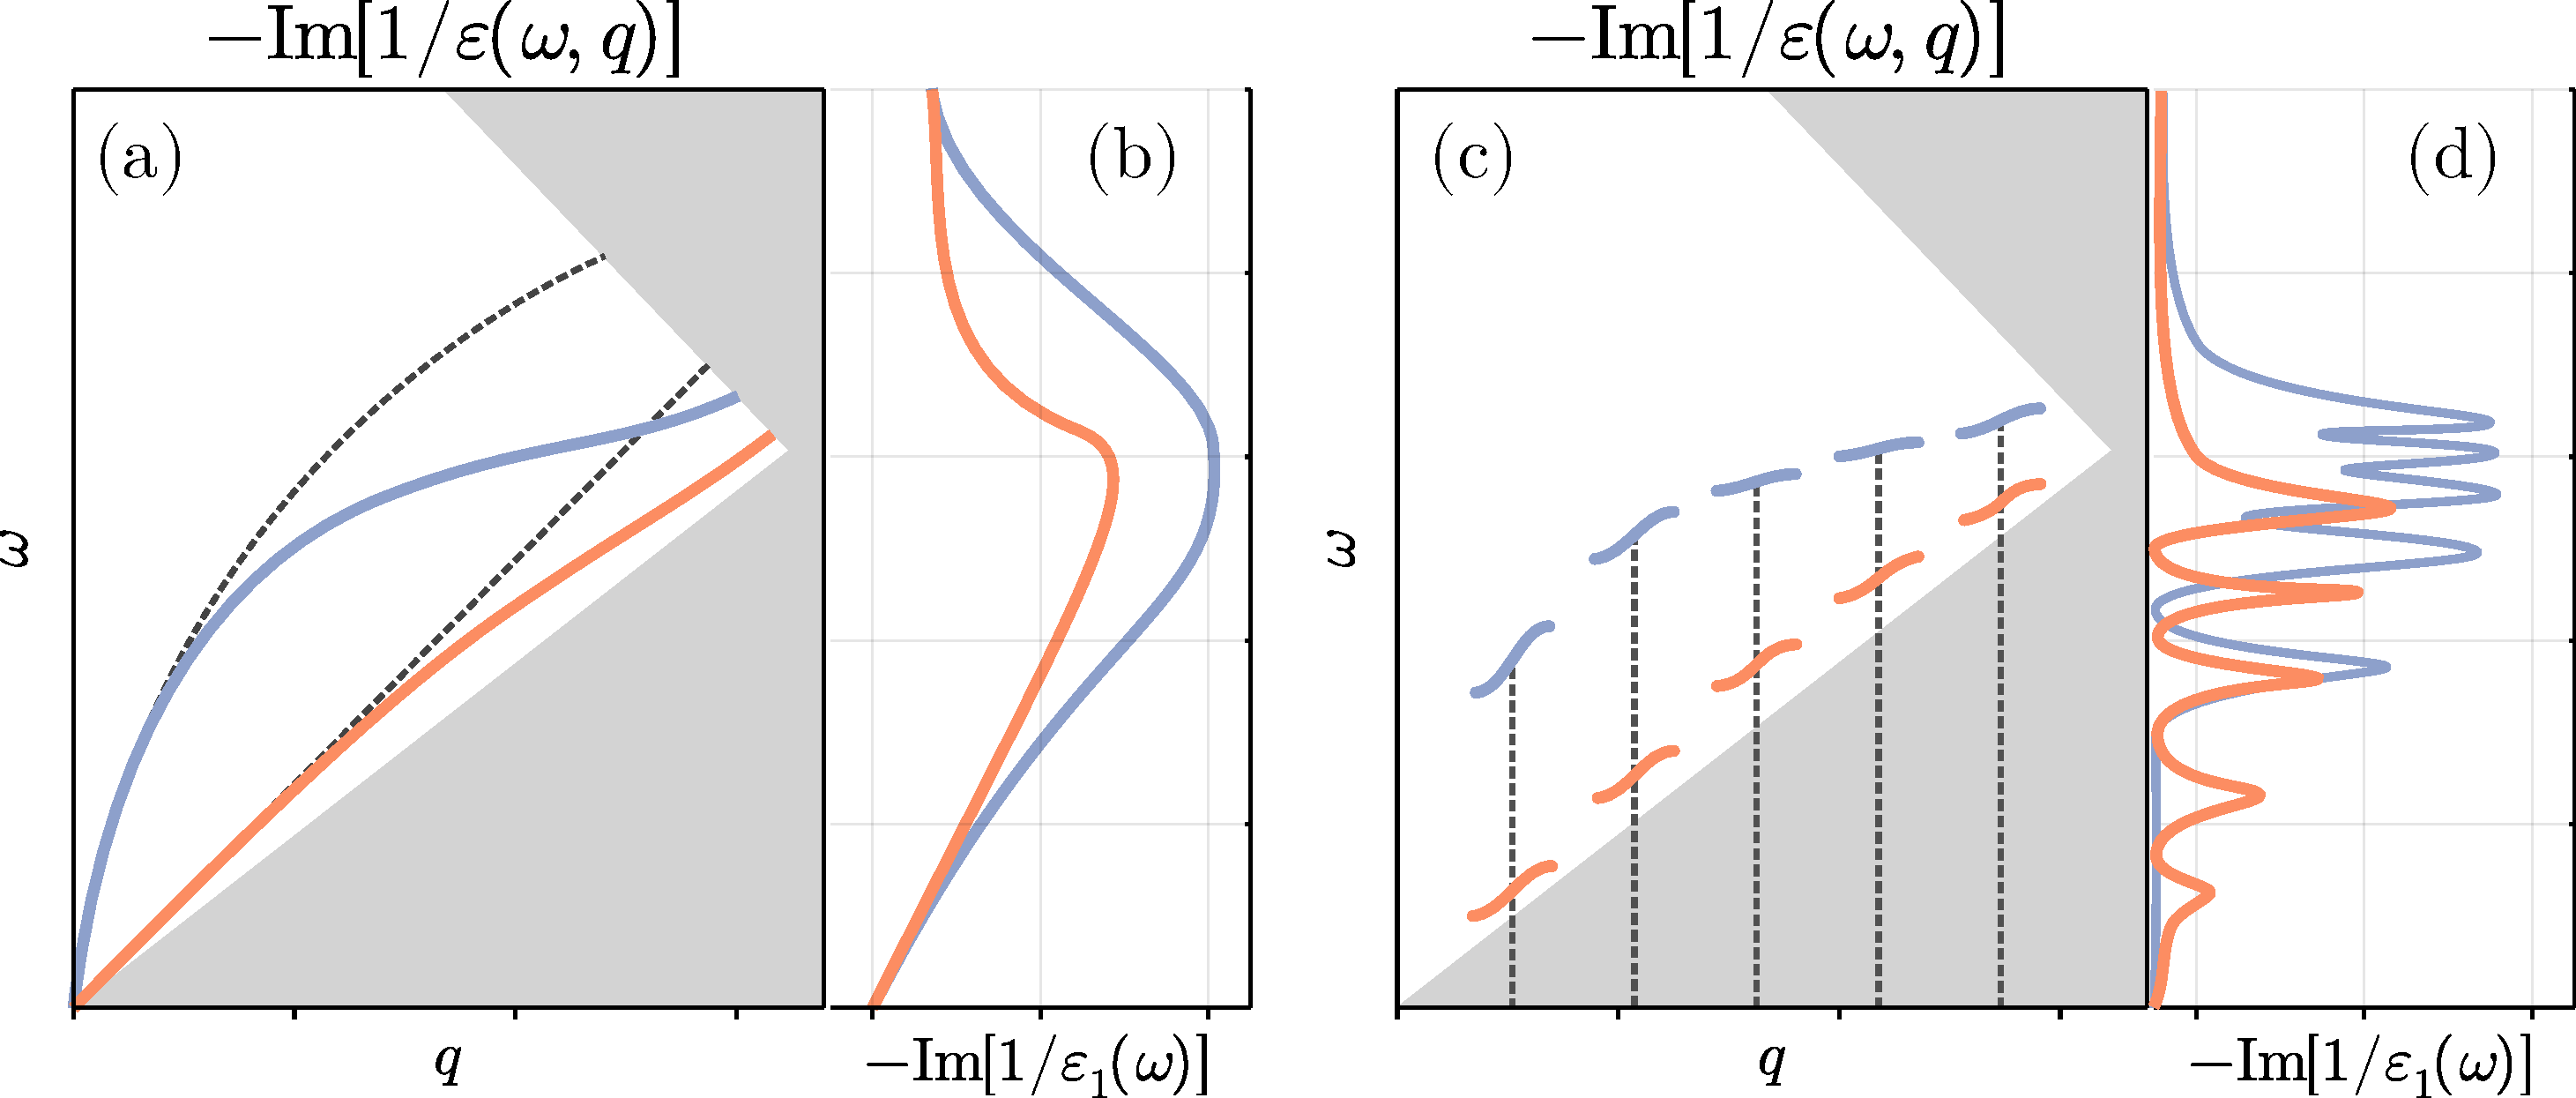
\includegraphics[width=0.8\textwidth]{handmade/Figure_4.pdf}
    \caption{Sketches of the qualitative plasmonic dispersion in pristine bilayer graphene a) together with the resulting plasmonic spectral functions b). The lower and upper grey triangles in a) represent the intra- and inter-band polarization continua. In c) and d) we sketch the same situation but for a finite-size system in which the momentum $q$ is discretized. \label{fig:mat22:BLGDispersion}}
\end{figure}

In the finite-size bilayer graphene supercells under consideration here, these plasmonic properties are modified as skeched in Fig.~\ref{fig:mat22:BLGDispersion}~c). The finite diameter of the hexagonal supercells defines an upper plasmonic wavelength $\lambda_\text{max}$ and a minimal wave vector $q_\text{min} \propto \lambda_\text{max}^{-1}$. Below this $q_\text{min}$ the system cannot host any of the plasmonic excitations of the $\omega_{\pm}(q)$ branches. Furthermore, the finite system size also discretizes the allowed momenta in multiples of this $q_\text{min}$. As a result the plasmonic dispersions become gapped between these $q$ values, and the full plasmonic spectrum becomes discretized as well, as sketched in Fig.~\ref{fig:mat22:BLGDispersion}~c),d). The previously continuous plasmonic spectrum now shows well defined discretized levels.

This is in full analogy to the formation of electronic quantum dot states: the finite system size discretizes the continuous electronic spectrum into well defined electronic quantum dot states. Based on this analogy, we call the resulting plasmonic states in the finite-size cells \emph{plasmonic quantum dot states}.  Their tunability is, however, much richer than in the case of electronic quantum dots. The energies of the plasmonic quantum dot states are controlled by a) the system size as this affects $q_\text{min}$, b) the doping level and substrate screening as this controls the energies of the underlying continuous branches $\omega_{\pm}(q)$, as well as by c) the twisting angle, as we will discuss in more detail in the following. Also the discretization of the linear $\omega_-(q)$ branch yields a very different level spacing than the discretized $\omega_+(q)$ branch as indicated in Fig.~\ref{fig:mat22:BLGDispersion}~d).

In the following sections we discuss how this scheme is realized in full real-space RPA calculations for finite AB-stacked (and twisted) bilayer graphene supercells.
    
\subsection{Plasmonic quantum dots in AB-stacked graphene supercells}
    
\begin{figure}
    \centering
    \subimport{assets}{Figure_5.pgf}
    % \includegraphics[width=0.99\columnwidth]{chapters/2D_Materials_9_1_014004/assets/Figure_5.png}
    \caption{a) Plasmonic dispersion for a supercell with diameter $d=150$\AA\ ($11028$ atoms). b), c) Plasmonic dispersion for a supercell with diameter $d\approx80$\AA\ ($3252$ atoms) together with full EELS($\omega$). Annotations in panel c) refer to subplots of Fig.~\ref{fig:mat22:modes}.}
    \label{fig:mat22:EELS}
\end{figure}
        
We start our discussion with comparing EELS($\omega,q$) for different finite-size supercells of untwisted AB-stacked bilayer graphene, which is defined by
\begin{equation*}
    \operatorname{EELS}(\omega, q) = -\operatorname{Im}\left[ \frac{1}{\varepsilon(\omega, q)} \right] \,,
\end{equation*}
where $\varepsilon(\omega, q)$ is the diagonal of the formal Fourier transform of $\varepsilon_{ij}(\omega)$. In Fig.~\ref{fig:mat22:EELS}~a) and b) we show EELS($\omega,q$) for hexagonal supercells of diameter $d=150$\AA\ ($11028$ atoms) and $d\approx80$\AA\ ($3252$ atoms), respectively. In both cases the electron doping is about $n = 5.3\times10^{14}\,$cm$^{-2} = 1.34\,$eV, which is around the maximum of what is achievable with double sided ionic-liquid gating techniques~\cite{zheliuk_josephson_2019}. In both of these panels we can clearly identify the $\omega_\pm(q)$ branches. In the case of the larger supercell we find a nearly continuous $\omega_+(q)$ branch, which starts to deviate from the $\sqrt{q}$ form around $q\approx 0.05\,$\AA$^{-1}$ showing the characteristic flattening. The lower $\omega_-(q)$ branch shows its approximate linear dispersion. For $q >0.2\,$\AA$^{-1}$ (above $\omega \approx 2.0\,$eV) both branches smear out due to strong Landau damping induced by the particle-hole continuum. Also note that the approximate plasmonic energies are similar to the ones observed in highly doped graphene monolayers~\cite{shin_control_2011}. Hence, the overall characteristics of these plasmonic branches are fully in line with the theoretical expectations as discussed in Sec.~\ref{sec:mat22:from-continuous-plasmon}, underlining the appropriateness of our modeling scheme. For the larger supercell only the lower branch shows first signs of discretization, which becomes more evident for the smaller cell in Fig.~\ref{fig:mat22:EELS}~b). In this case we find clear gaps in both branches, which is also reflected in the discrete peaks in the full EELS($\omega$) depicted in Fig.~\ref{fig:mat22:EELS}~c).

\begin{figure}
    \centering
    \subimport{./assets}{Figure_6.pgf}
    % \includegraphics[width=0.7\columnwidth]{chapters/2D_Materials_9_1_014004/assets/Figure_6.png}
    \caption{Plasmonic eigenmodes in real space for a supercell with $3252$ atoms. Depicted modes correspond to the highlighted excitation energies in Fig.~\ref{fig:mat22:EELS}~c).}
    \label{fig:mat22:modes}
\end{figure}

From the comparison between the momentum resolved EELS($\omega,q$) with the plasmonic levels in the full EELS($\omega$), we can identify the origin of the specific plasmonic states. Starting at the lowest level with $\omega \approx 0.32\,$eV [barely visible in Fig.~\ref{fig:mat22:EELS}~c)] we see that this mode arises from the layer polarized $\omega_-(q)$ branch. %[black dashed line in Fig.~\ref{fig:mat22:EELS}~b),c)].
The corresponding layer-resolved real-space representation of that mode (the eigenvector $\phi_1(r, \omega\approx 0.32\,$eV$)$ of the dielectric function) is shown in Fig.~\ref{fig:mat22:modes}~a). As expected, we find a layer-polarized excitation with a homogeneous charge distribution within each layer.  The next plasmonic level at $\omega \approx 0.63\,$eV is again resulting from the $\omega_-(q)$ branch, which accordingly shows the layer polarization, see Fig.~\ref{fig:mat22:modes}~c). However, the charge distribution within each layer is not homogeneous anymore and this mode is best described as a layer-polarized dipole excitation. It is accompanied at the same $q$ by a plasmonic excitation with $\omega \approx 1.2\,$eV, which originates from the upper $\omega_+(q)$ branch.
%[blue dashed lines in Fig.~\ref{fig:mat22:EELS}~(b,c)].
Accordingly, this mode does not show a layer polarization [Fig.~\ref{fig:mat22:modes}~c)], but is otherwise also of dipole character. The plasmonic mode at $\omega \approx 1.0\,$eV is again originating from the layer polarized branch, as is also evident from its real-space representation depicted in Fig.~\ref{fig:mat22:modes}~e). This mode has a circular charge distribution, which is vastly reminiscent of a $1s$ atomic wave function. This mode is as well accompanied at the same $q$ by a $1s$-like plasmonic state at $\omega \approx 1.65\,$eV from the upper branch,% [orange dashed-doted line in Fig.~\ref{fig:mat22:EELS} (b,c)],
which does not show any layer polarization. Finally, we find another layer-polarized plasmonic excitation around $\omega \approx 1.3\,$eV which hosts a $p$-like state [see Fig.~\ref{fig:mat22:modes}~f)] which is again reminiscent of the atomic-like wave functions of electronic quantum dots. For this mode, we were however not able to identify the accompanying mode from the upper plasmonic branch, which we attribute to smaller energy separation of plasmonic states at higher energies, as also indicated in the sketches in Fig.~\ref{fig:mat22:BLGDispersion}.

Thus, next to the finite-size induced discrete energy levels and tunability, these plasmonic charge distributions can also resemble atomic-like wave functions of electronic quantum dots, which further underlines their identification as plasmonic quantum dots. In the following we proceed with the twist-angle dependence, focusing on the dipole and $1s$-like modes.

\subsection{Twist angle dependence}

\begin{figure*}
    \centering
    \subimport{./assets}{Figure_7.pgf}
    % \includegraphics[width=0.9\textwidth]{chapters/2D_Materials_9_1_014004/assets/Figure_7.png}
    \caption{Plasmonic eigenmodes in real space for various twisting angles $\theta=0\degree,\,10\degree,\,20\degree,\,30\degree$. Columns show evolution of different modes: a) ``dark'' dipole, b) ``bright'' dipole, c) ``dark`` $1s$, d) ``bright'' $1s$.}
    \label{fig:mat22:modesTheta}
\end{figure*}

From the previous discussion, the dependence of the plasmonic quantum dot energies on doping level and system size are already clear. In the following we thus focus on the twist angle dependence. To this end we present in Fig.~\ref{fig:mat22:modesTheta} the ``dark'' and ``bright'' dipole and $1s$ modes for $\theta=0\degree, \,10\degree, \,20\degree, \,30\degree$. Modes are called ``dark'' or ``bright'' when they originate from $\omega_-(q)$ or $\omega_+(q)$ branches, respectively.

For the bright dipole modes, shown in Fig.~\ref{fig:mat22:modesTheta}~b), we observe that the boundary separating the differently charged areas is rotating when we adjust $\theta$, synchronously in the lower and upper layer, however, only with $\theta/2$. The latter can be readily understood by overlaying the rotated dipole patterns and by remembering that the charge distributions in the two layers are not independent. The missing overlap at the corners of the hexagons additionally yields enhanced charge accumulations in the two opposite corners of each layer. The dark dipole mode, shown in Fig.~\ref{fig:mat22:modesTheta}~a), behaves similarly. The charge separation line again rotates with $\theta/2$, but we observe a smearing of it, such that the charge separation is not as sharp as in the bright dipole mode. Note that rotated dark dipole modes are additionally rotated by $90\degree$ compared to $\theta=0\degree$ case. This, however, does not affect any of the drawn conclusions as these unrotated dipole modes have nearly the same excitation energies.%, see Fig.~\ref{fig:mat22:doping} for more details.

In Fig.~\ref{fig:mat22:modesTheta}~c) and d), we depict patterns of the $1s$ quantum dot mode. Except for a slight deformation of the initial hexagonal shape we do not see any major changes to the bright excitation upon twisting. Its dark counterpart also does not show any significant changes in its excitation pattern, except for a smearing of the clear charge separation.

\SideFigure{0.42\textwidth}{0pt}{0.4\textwidth}{\subimport{./assets}{Figure_8.pgf}%
}{Excitation energies of all modes from Fig.~\ref{fig:mat22:modesTheta} as a function of $\theta$.%
}{fig:mat22:ex_vs_deg}

In fact, the most important changes to these plasmonic states are their excitation energy shifts. In Fig.~\ref{fig:mat22:ex_vs_deg} we plot the excitation energies for all modes as a function of $\theta$. We see that within the given accuracy, the excitation energies of the bright modes do not depend on the rotation angle. The dark modes, however, do. We see for both the dark dipole and the dark $1s$ mode that the energy is significantly decreased upon $10$ degree twist. Afterwards, these modes just mildly depend on further rotation towards $\theta=30\degree$. The initial symmetry breaking between $0\degree$ and $10\degree$ thus leaves the strongest footprint in the plasmonic energies, while the larger rotation angles do not change it too drastically anymore. 

We attribute this different impact of the rotation to the bright and dark modes to the single-particle properties. In Fig.~\ref{fig:mat22:BLGDispersion}, the original continuous ``bright'' plasmonic branch $\omega_+(q)$ is clearly detached from the particle-hole continuum (shown in grey), while the ``dark'' $\omega_-(q)$ branch is in its close vicinity. Thus, the dark states are much more prone to Landau damping and to changes in the particle-hole continuum due to modifications of the the single-particle electronic states. 

To verify this hypothesis we calculated EELS($\omega$) for
\begin{equation*}
    \varepsilon(\omega, \theta, \alpha) = 1 - U(\alpha) \Pi^{p_z}(\omega, \theta),
\end{equation*}
where $\theta$ and $\alpha$ are both referring to the twist angle, but now separated in the rotation in the polarizability ($\theta$) and the Coulomb interaction ($\alpha$) matrices. For all previous calculations we have set $\alpha = \theta$.
From the resulting spectra (see Supplemental Information), % in Fig.~\ref{fig:mat22:RotEELS}
we see that the rotation in the Coulomb interaction matrix, in other words changes to $\alpha$, barely affect the energy of the dark $1s$ mode, whereas the rotation in the polarizability matrix (changes to $\theta$), strongly affect it.
Thus, indeed the single-particle properties as reflected by the polarizability affect the dark states the most. If we additionally remember that the \emph{approximate} moir\'{e} lattice constant $\lambda$ is inversely proportional to $\sin(\theta/2)$, yielding $\lambda(\theta=10\degree) \approx 14\,$\AA, $\lambda(\theta=20\degree) \approx 8\,$\AA, and $\lambda(\theta=30\degree) \approx 6\,$\AA, we understand that the changes to the lattice structure are the largest when going from $\theta=0\degree$ to $\theta=10\degree$, while increasing $\theta$ further modifies $\lambda$ only slightly. Under a reasonable assumption that changes to the lattice structure are also imprinted on the electronic structure, we can qualitatively understand why the excitation energy of the dark modes is affected the most upon the initial twist by $\theta=10\degree$.

\section{Conclusions \& outlook}
    
We have presented an ab initio derived twisted bilayer graphene many-body model including a consistent description of the kinetic (hopping) and Coulomb matrix elements. Upon separating the different screening channels into the low-energy $p_z$ and residual background screening, we were able to map the twisting dependence of the total polarizability to the low-energy screening channels only. This allowed us to calculate the background-screened Coulomb interaction from first principles using constrained RPA and to fit the resulting partially-screened interaction with a lightweight continuous model. All rotation dependencies were subsequently handled within the low-energy $p_z$ subspace only. 

Based on this model we studied low-energy plasmonic excitations in real space in electron-doped twisted bilayer graphene supercells. We found that the system-size-induced discretization of the plasmonic spectrum gives rise to plasmonic quantum dot states, which can be tuned by the doping level, system size, and, as we have discussed in detail, by the twisting angle. In fact, we showed that two different types of plasmonic quantum dot states arise from the two plasmonic branches of pristine bilayer graphene. These differ in their layer polarization. Layer-polarized states are strongly affected by twisting, whereas their in-phase counterparts are almost completely twist-independent.

Since plasmonic quantum dot modes are highly inhomogeneous due to their real-space confinement as well as due to their different in- and out-of-plane structures (dipole-, $1s$-, $1p$-like) they can couple to external electromagnetic fields~\cite{crowell_surface-plasmon_1970,maradudin_scattering_1975}. In combination with a high degree of tunability, this allows for very promising light-matter engineering routes within sensors, diodes, or photovoltaic applications. In this respect, we would like to emphasize that for the chosen system size and doping levels, the plasmonic energies already lie in the visible / near-infrared range. 

For the characterization of these plasmonic quantum dot modes, we imagine scanning near-field optical microscopy measurements~\cite{fei_gate-tuning_2012,chen_optical_2012} as most promising, as they allow spatial mapping of charge distributions.

We thus expect that this initial study forms the ground for further material-specific quantitative real-space plasmonics studies of twisted bilayer graphene and similar systems.

\section{Additional resources}

\QRListItem{https://github.com/twesterhout/graphene-plasmons}{Code to perform the analysis in this chapter is available on GitHub.}
\QRListItem{https://github.com/twesterhout/Plasmons.jl}{Julia implementation of the real-space RPA method. Also available on GitHub. The code runs on both CPUs and GPUs.}
\QRListItem{https://doi.org/10.5281/zenodo.14993548}{Zenodo dataset with data to reproduce all figures in this chapter. The figures can be re-generated by running \texttt{nix build github:twesterhout/phd-thesis\#Materials\_9\_1\_014004}.}
\QRListItem{https://iopscience.iop.org/article/10.1088/2053-1583/ac38ca/meta\#tdmac38caapp1}{Appendices covering doping dependence, ab initio details, RPA details, and more data on $\alpha$ dependence.}
%   \section*{Appendix}

%       \subsection{Doping dependence \label{sec:app_doping}}

%        \begin{figure}
% 	\includegraphics[width=0.99\columnwidth]{../assets/Figure_9.png}
% 	\caption{
% 	    Classical and quantum dot plasmonic modes in real-space for $\theta = 0\degree$ together with their excitation energies at reduced doping ($\mu = 0.2$ eV). Panels (a) and (b) depict ``bright'' and ``dark'' modes respectively. Modes in panel (b) are half-transparent to indicate that they are not real plasmonic eigenmodes (the condition $\mathrm{Re}[\varepsilon(\omega)] = 0$ is not satisfied).
% 	    \label{fig-doping}
% 	}
% \end{figure}

% In Fig.~\ref{fig-doping} we present a few plasmonic excitation patterns for a smaller electron doping of $n = 6.3\times10^{13}\,\mathrm{cm}^{-2} = 0.2\,\mathrm{eV}$ and the same supercell as before. In this case we can again clearly identify a variety of bright modes. The dark modes are, however, not well defined anymore. Although we find some plasmonic eigenvectors which resemble the corresponding dark modes at lower excitation energies, these are not well defined plasmonic excitations since the real part of the dielectric function does not fulfill the necessary requirement $\operatorname{Re}\left[ \varepsilon(\omega) \right] = 0$. The excitation energies of the bright dipole and $1s$ modes are strongly reduced compared to the corresponding mode at high electron doping. These observations are in line with the expected behaviour of the previously mentioned $\omega_{\pm}(q)$ modes~\cite{das_sarma_plasmons_1998,hwang_plasmon_2009,roldan_dielectric_2013}. 
% The vanishing / fading of the dark modes is thus a result of their close vicinity to the electron-hole continuum.

%       \subsection{Ab initio details \label{sec:app_ab}}

%       Our ab initio calculations were performed within density functional theory utilizing the projected augmented wave (PAW) formalism~\cite{paw1, paw2} as implemented in the \emph{Vienna ab initio simulation package} ({\sc vasp})~\cite{Kresse1, Kresse2}. The exchange-correlation effects were considered using the generalized gradient approximation (GGA)~\cite{gga}. A $517\,$eV energy cut-off for the plane-waves and a convergence threshold of $10^{-7}\,$eV were used in the calculations. The Brillouin zone was sampled by a ($18 \times 18$) ${\bf  k}$-point mesh. The in-plane lattice constant was set to $2.468\,$\AA\ and the out-of-plane distance between the two layers was $3.35\,$\AA. A $25\,$~\AA-thick super-cell was used in the direction orthogonal to the 2D plane in order to reduce spurious interactions between supercell images.
%       The Wannier functions and the tight-binding Hamiltonian were calculated within the scheme of maximal localization~\cite{mlwf1,mlwf2} using the {\sc wannier90} package~\cite{wannier90}. Therefore, we used an inner (frozen) wannierization windows of about $4.5\,$eV around the Fermi level. This way the Wannier-interpolated band structure perfectly reproduces the Kohn-Sham states within this window and shows only minor deviations away from it.
    
%       The Coulomb interaction was evaluated using the maximally-localized Wannier functions within the constrained Random Phase Approximation (cRPA)~\cite{CoulombU, KaltakcRPA} as ${U_{ij}=\langle w_i w_j |U|w_j w_i\rangle}$, where $U$ was the partially-screened Coulomb interaction defined by ${U=v+v \Pi^\text{rest} U}$ with $v$ --- the bare Coulomb interaction, $\Pi^\text{rest}$ --- the cRPA polarizability, and $w_i$ --- the Wannier function at lattice site $i$. The polarizability operator $\Pi^\text{rest}$ describes screening from all electronic states except those given by the tight-binding Hamiltonian in the Wannier basis. For these calculations, we used a recent cRPA implementation by Kaltak within {\sc vasp}~\cite{KaltakcRPA}. To converge the cRPA polarization with respect to the number of empty states we used in total $208$ bands.
    
%       \subsection{RPA details \label{sec:app_rpa}}
    
%       The screening from the low-energy $p_z$ orbitals is calculated using the real-space Random Phase Approximation code from Ref.~\cite{westerhout_plasmon_2018}. This code evaluates Eq.~\eqref{eqn-Pi_pz} for a given single-particle Hamiltonian at a given temperature $T$ and damping $\eta$. In all our calculations, the temperature was set to $k_\mathrm{B} T = 0.0256$ eV and damping was $\eta = 0.001$ eV. Compared to Ref.~\cite{westerhout_plasmon_2018} we applied two notable optimizations. First of all, we reduced the comutational load by taking the sparsity of Eq.~\eqref{eqn-Eps_pz} at finite temperatures into account. This reduced the effective algorithmic complexity from $\mathcal{O}(N^4)$ to $\mathcal{O}(N^{3.13})$ where $N$ was the number of lattice sites. Furthermore, we run the computations on Graphics Processing Units (GPUs) which are much better at dense linear algebra than CPUs. All together, we could evaluate Eq.~\eqref{eqn-Pi_pz} for a given $\omega$ in less than 30 seconds on an NVIDIA V100, whereas for a comparable system size it took more than 24 hours in Ref.~\cite{westerhout_plasmon_2018}, thus achieving $\times 3000$ speedup.
    
%       An example of a resulting polarizability function in real space is depicted in Fig.~(\ref{fig-Coulomb}).
    
%       \begin{figure}
%           \includegraphics[width=0.9\columnwidth]{../assets/Figure_10.png}
%           \caption{%
%               Static polarizability $\Pi^{p_z}(r, r', \omega=0)$ for two different choices of $r'$. The color bar is clamped to a small range to highlight the oscillating tails.
%               \label{fig-Coulomb}
%           }
%        \end{figure}
     
%        \subsection{Rotation Details}
     
%        In Fig.~(\ref{fig-RotEELS}) we show EELS($\omega$) around the unrotated and $10\degree$-rotated dark $1s$ mode energies for individual rotations of the involved Coulomb ($\alpha$) and polarizability ($\theta$) matrices. From this, it is evident that the rotation of the polarizability matrix affects EELS the most.
     
%       \begin{figure}
%           \includegraphics[width=0.9\columnwidth]{../assets/Figure_11.pdf}
%           \caption{%
%               EELS($\omega$) around the unrotated and $10\degree$-rotated dark $1s$ mode energies for individual rotations of the involved Coulomb ($\alpha$) and polarizability ($\theta$) matrices.
%               \label{fig-RotEELS}
%           }
%        \end{figure}

%   \bibliography{lib.bib}
